\documentclass[12pt]{article}
\usepackage[a4paper, total={6in, 9in}]{geometry}
\usepackage{graphicx}
\graphicspath{ {./images/output/} }
\usepackage{caption}
\usepackage[english]{babel}
\usepackage{titling}
\usepackage{float}
% \usepackage{amsmath}
% \usepackage{minted}
% \usepackage{multicol}
% \usepackage{array}
% \usepackage{setspace}
% \usepackage{placeins}
\setlength{\parindent}{0pt}

% \usepackage{lipsum}

\title{Demonstration of AutoCAD Tools and DOL Starter Diagram}
\author{}
\date{}

\pagenumbering{gobble}
\begin{document}
\vspace*{\fill}
\begin{center}

    \emph{Heaven's Light is Our Guide} \\
    \textbf{Rajshahi University of Engineering and Technology} \\

    \begin{figure}[H]
        \centering
        
\includegraphics[scale=.34]{images/RUET_logo.png}
        \label{fig:ruet_logo}
    \end{figure}
    \vspace{5mm}

    \textbf{Course Code}\\
    ECE 3200\\
    \vspace{3mm}
    \textbf{Course Title}\\
    Electrical Services Design

    \vspace{5mm}
    \textbf{Experiment Date:} {February 4, 2025}\\
    \textbf{Submission Date:} {February 18, 2025}\\

    \vspace{5mm}
    \textbf{Lab Report 5: \\ Implementation of Parametric \& Full Units PLC: Insertion, Editing, \& Modification.}

    \vspace{15mm}

    \begin{tabular}{c|c}
        \textbf{Submitted to} & \textbf{Submitted by} \\
        Md. Faysal Ahamed     &                       \\
        Lecturer              &                       \\
        Dept of ECE, RUET     & Md. Tajim An Noor     \\
        -                     & Roll: 2010025         \\
        Moloy Kumar Ghosh     &                       \\
        Lecturer              &                       \\
        Dept of ECE, RUET     &                       \\
    \end{tabular}

\end{center}
\vspace*{\fill}


\pagebreak

\tableofcontents

\pagebreak
\pagenumbering{arabic}
\maketitle

\section*{Introduction}
\addcontentsline{toc}{section}{Introduction}
AutoCAD Electrical is a specialized software application designed to streamline electrical design workflows by offering an array of powerful tools tailored for creating and managing electrical schematics. It is widely used in industries for designing control systems, electrical circuits, and panel layouts. The software provides enhanced precision, automation, and efficiency, making it an essential tool for modern electrical engineering projects.\\\\
This report explores the key functionalities of AutoCAD Electrical, including the use of snap tools, ladder diagram creation, and grid and zone setup. Snap tools are essential for ensuring that components and wires are precisely aligned, which is crucial for maintaining the accuracy of electrical schematics. Ladder diagram creation allows for the systematic representation of electrical circuits, making it easier to design and troubleshoot control systems. Grid and zone setup helps in organizing the workspace and ensuring that the design adheres to industry standards.
\\\\
Additionally, the report covers the design of a 3-phase Direct-On-Line (DOL) motor circuit using AutoCAD Electrical. This involves creating detailed drawings of the motor circuit without simulation, focusing on the practical aspects of using the software tools. By delving into these topics, the report highlights the capabilities of AutoCAD Electrical in addressing real-world electrical design challenges and provides a comprehensive understanding of the tools used in this experiment.

\section*{Required Equipment/Software}
\addcontentsline{toc}{section}{Required Equipment/Software}
\begin{itemize}
    \item AutoCAD Electrical
    \item \LaTeX{} for report writing
\end{itemize}

\section*{Tools and Techniques}
\addcontentsline{toc}{section}{Procedure}
\subsection*{Snap Options}
\addcontentsline{toc}{subsection}{Snap Options}
The Snap Tool in AutoCAD ensures precision by allowing the cursor to jump to specific points on objects or along a grid. Key snap options include:

\begin{itemize}
    \item \textbf{Endpoint Snap}: Snaps to endpoints of lines, arcs, splines, or polylines.
    \item \textbf{Midpoint Snap}: Snaps to the exact midpoint of a line, arc, or polyline segment.
    \item \textbf{Center Snap}: Snaps to the center of a circle, arc, or ellipse.
    \item \textbf{Node Snap}: Snaps to point objects, such as points or block insertion points.
    \item \textbf{Quadrant Snap}: Snaps to the four quadrants (0°, 90°, 180°, 270°) of a circle, arc, or ellipse.
    \item \textbf{Intersection Snap}: Snaps to the intersection point of two objects.
    \item \textbf{Extension Snap}: Extends a line beyond its endpoint and snaps to an extrapolated point.
    \item \textbf{Insertion Snap}: Snaps to the insertion point of a block or text.
    \item \textbf{Perpendicular Snap}: Snaps to a point perpendicular to another object.
    \item \textbf{Tangent Snap}: Snaps to a point tangent to a circle, arc, or ellipse.
    \item \textbf{Nearest Snap}: Snaps to the nearest point on an object.
    \item \textbf{Apparent Intersection Snap}: Snaps to the apparent intersection of two objects in 3D space.
    \item \textbf{Parallel Snap}: Snaps to create a line parallel to another existing line.
    \item \textbf{Geometric Center Snap}: Snaps to the geometric center of a closed polyline or spline.
    \item \textbf{None Snap}: Disables snapping temporarily.
\end{itemize}

Enable/Disable Snap Options:
\begin{itemize}
    \item \textbf{Command:} OSNAP - Opens the Object Snap Settings dialog box.
    \item \textbf{Shortcut Menu:} Right-click the Snap Mode icon in the status bar and select the desired snap options.
\end{itemize}

\addcontentsline{toc}{section}{Output}
\begin{figure}[H]
    \centering
    \begin{minipage}{0.45\textwidth}
        \centering
        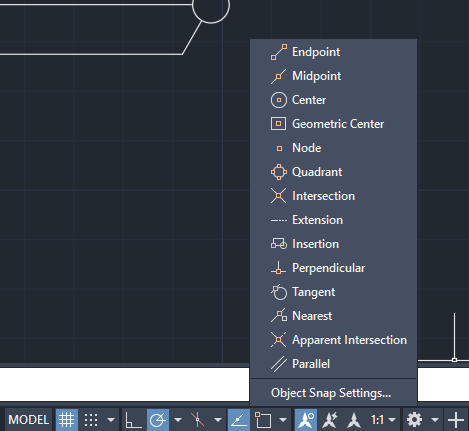
\includegraphics[width=\textwidth]{snap.png}
        \caption{Snap Options in AutoCAD Electrical}
        \label{fig:snap_options}
    \end{minipage}\hfill
    \begin{minipage}{0.45\textwidth}
        \centering
        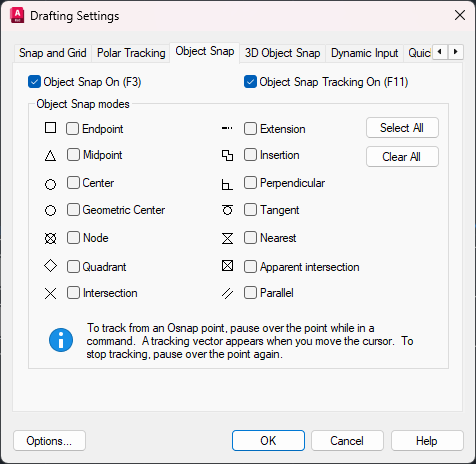
\includegraphics[width=\textwidth]{draft.png}
        \caption{Drafting settings in AutoCAD Electrical}
        \label{fig:draft_settings}
    \end{minipage}
\end{figure}

\subsection*{Ladder Diagram Settings}
\addcontentsline{toc}{subsection}{Ladder Diagram Settings}
\begin{itemize}
    \item \textbf{Inserting a Ladder:}
          \begin{itemize}
              \item Use the "Insert Ladder" command from the Schematic tab.
              \item Specify the ladder parameters like the number of rungs, spacing, and reference numbers, then place the ladder in the drawing.
          \end{itemize}
    \item \textbf{Renumbering the Ladder:}
          \begin{itemize}
              \item Use the "Renumber Ladder Rungs" command.
              \item Select the ladder, and AutoCAD Electrical will automatically update the rung numbers sequentially based on your settings.
          \end{itemize}
    \item \textbf{Repositioning the Ladder:}
          \begin{itemize}
              \item Use the "Move Ladder" command to select and reposition the entire ladder.
              \item Drag the ladder to the desired location while keeping its structure intact.
          \end{itemize}
    \item \textbf{Changing Rung Spacing:}
          \begin{itemize}
              \item Use the "Edit Ladder" command and modify the rung spacing parameter.
              \item The ladder will automatically update to reflect the new spacing without altering the rung numbers.
          \end{itemize}
\end{itemize}

\addcontentsline{toc}{section}{Output}
\begin{figure}[H]
    \centering
    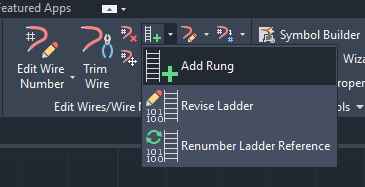
\includegraphics[width=.5\textwidth]{rung.png}
    \caption{Ladder Diagram Settings in AutoCAD Electrical}
    \label{fig:ladder_settings}
\end{figure}

\subsection*{X-Y Grid Setup}
\addcontentsline{toc}{subsection}{X-Y Grid Setup}
\begin{itemize}
    \item Use the "Drawing Properties" or "Grid Setup" command to configure the X-Y grid.
    \item Define the horizontal (X) and vertical (Y) grid intervals and labels to suit your project layout.
\end{itemize}

\subsection*{X-Zones Setup}
\addcontentsline{toc}{subsection}{X-Zones Setup}
\begin{itemize}
    \item Use the "Insert Zones" command to set up zones along the X-axis.
    \item Specify the start and end coordinates, zone width, and labeling format, then place the zones on the drawing.
\end{itemize}

\addcontentsline{toc}{section}{Output}
\begin{figure}[H]
    \centering
    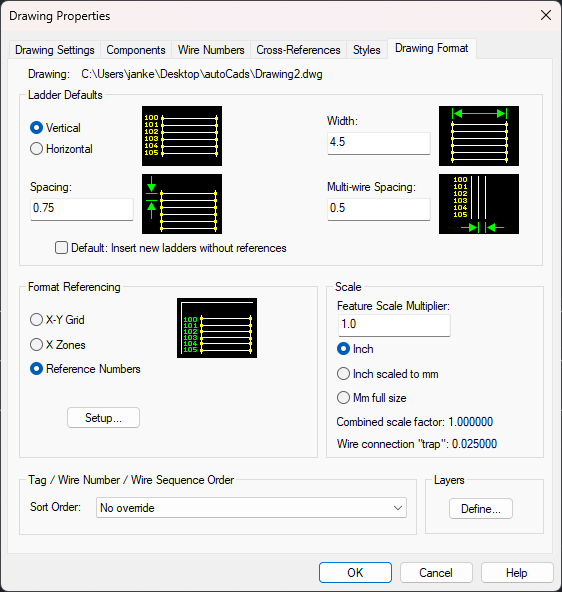
\includegraphics[width=.5\textwidth]{drawp.png}
    \caption{Drawing Properties and X-Zones Setup in AutoCAD Electrical}
    \label{fig:zones}
\end{figure}


\section*{Motor Circuit Design}
\addcontentsline{toc}{section}{Motor Circuit Design}
A Direct-On-Line (DOL) motor starter is a straightforward and cost-effective method to start electric motors. It directly connects the motor to the full line voltage, providing maximum torque during startup. A DOL starter typically includes:

\begin{itemize}
    \item \textbf{Circuit Breaker or Fuse:} Provides protection against short circuits and overloads.
    \item \textbf{Contactor:} Acts as a switch to connect and disconnect the motor from the power supply.
    \item \textbf{Overload Relay:} Protects the motor from overheating by disconnecting it if it draws excessive current for a prolonged period.
\end{itemize}

DOL starters are primarily used for small motors where high inrush current during startup is acceptable. They are easy to design, operate, and maintain, making them a popular choice for basic motor control applications.

\section*{Output}
\addcontentsline{toc}{section}{Output}
\begin{figure}[H]
    \centering
    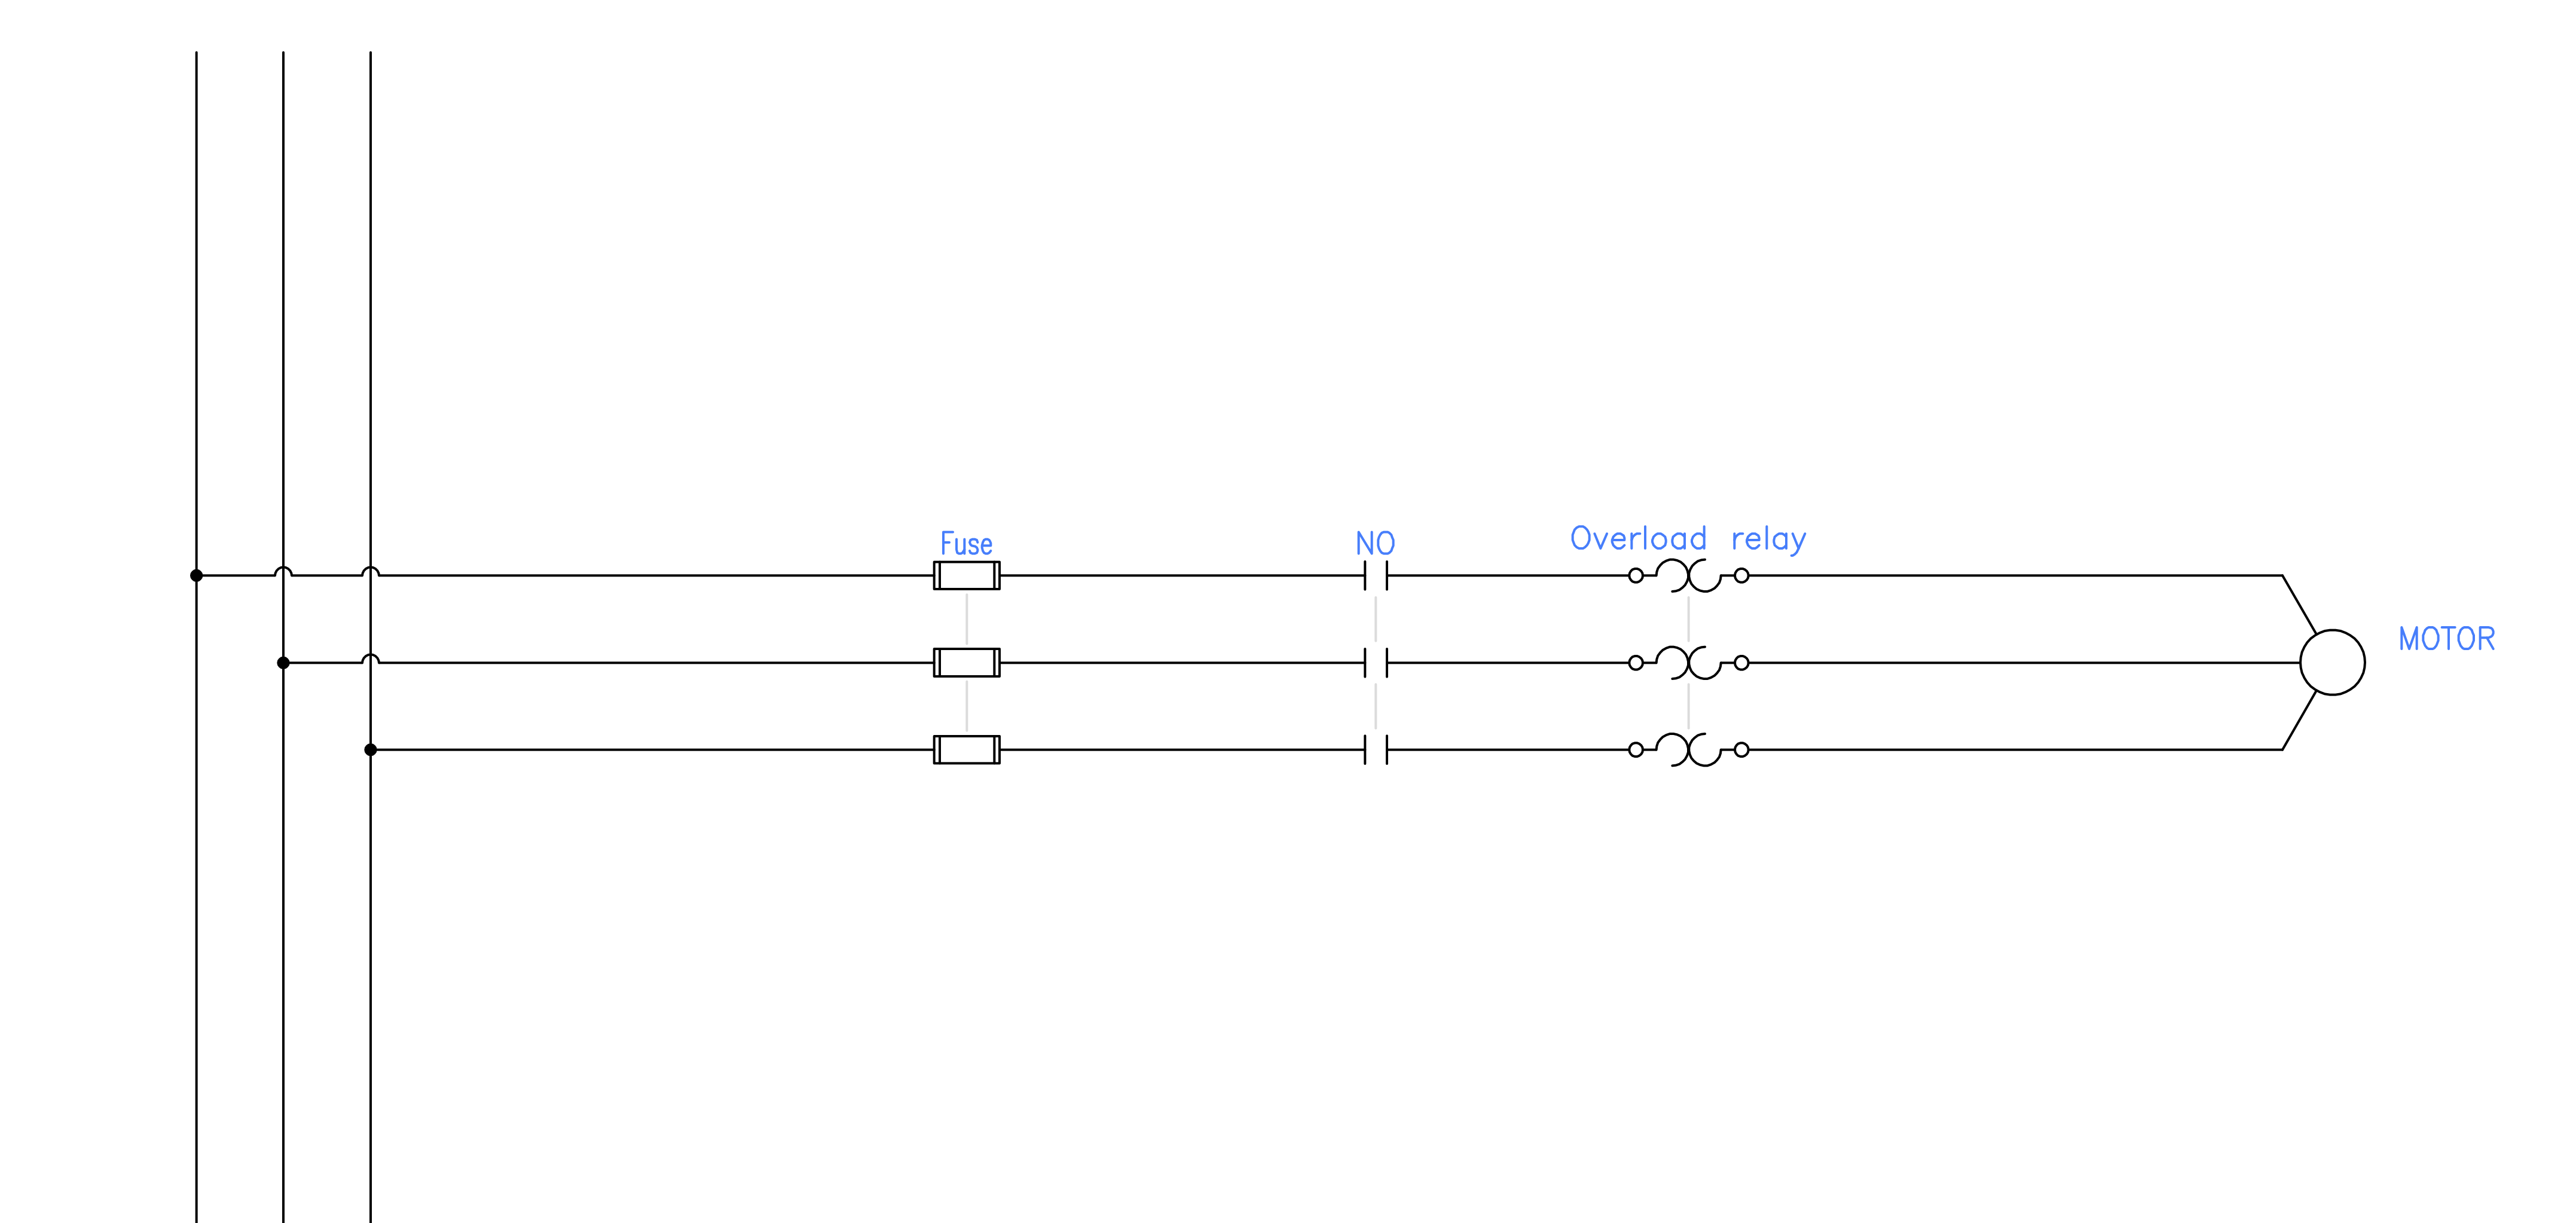
\includegraphics[width=.9\textwidth]{DOL.png}
    \caption{Ladder Diagram of a 3-phase DOL Motor Circuit}
    \label{fig:motor_circuit}
\end{figure}

\section*{Discussion \& Conclusion}
\addcontentsline{toc}{section}{Discussion \& Conclusion}
AutoCAD Electrical offers a comprehensive set of tools and features tailored for electrical design tasks. The snap options ensure precise alignment of components, while ladder diagram settings facilitate the systematic representation of electrical circuits. The X-Y grid and X-Zones setup help in organizing the workspace and adhering to industry standards.\\\\

% \bibliographystyle{IEEEtran}
% \renewcommand{\bibname}{References}
% \addcontentsline{toc}{section}{References}
% \bibliography{ref}

\end{document}
